\documentclass[10pt]{article}
\usepackage[margin=0.85in]{geometry}
\usepackage{amsmath,amssymb,graphicx,booktabs,array,xcolor,longtable,calc,etoolbox}
\usepackage[numbers,sort&compress]{natbib}
\usepackage[font=small,labelfont=bf]{caption}
\usepackage[colorlinks=true,allcolors=blue]{hyperref}
\hypersetup{pdftitle={Acephale V2: goal-conditioned speculative reads under exact-source constraints}}
\pdfinfoomitdate=1
\pdftrailerid{}
\setlength{\parindent}{0pt}
\setlength{\parskip}{3pt}
\setlength{\textfloatsep}{12pt plus 2pt minus 2pt}
\setlength{\floatsep}{10pt plus 2pt minus 2pt}
\setlength{\intextsep}{10pt plus 2pt minus 2pt}
\renewcommand{\topfraction}{0.85}
\renewcommand{\textfraction}{0.1}
\renewcommand{\floatpagefraction}{0.75}
\title{Acephale V2: goal-conditioned speculative reads under exact-source constraints}
\author{}
\date{23 November 2026}

\providecommand{\tightlist}{\setlength{\itemsep}{0pt}\setlength{\parskip}{0pt}}
\AtBeginEnvironment{longtable}{\small}
\setlength{\LTpre}{8pt}
\setlength{\LTpost}{8pt}

\begin{document}
\maketitle
\begin{center}\small Working paper. All failed, unavailable, censored and undispatched outcomes remain in their original denominators.\end{center}
\begin{abstract}
We study whether source-grounded goal inference can improve speculative tool reads for a fixed language-model actor. The design separates candidate availability, prediction, safe execution, and end-to-end task outcomes. A prospective research cohort contains 36 source-collection runs, 160 paired development trials, and a conditional 400-trial heldout stage. A separate native-prefix head experiment compares complete training recipes rather than isolating architecture. The original 132-trial fast-tool study remains an immutable negative control.

\textbf{Primary comparison unavailable.} The retained final analyzer reports development-gate passage as no. Unavailable, failed, censored and undispatched cases remain explicit. Report completion is not independently judged task success.
\end{abstract}

\hypertarget{question-and-mechanism}{%
\section{Question and mechanism}\label{question-and-mechanism}}

Goal conditioning can only help after an exact future read is represented in the current candidate set. The actor remains authoritative. Exact-request reuse targets latency while leaving the actor and its tool decisions fixed; it does not train the actor or directly establish improved decision quality. Candidates are read-only visit calls grounded in URLs from actual preceding search responses, linked by real tool-call IDs. Historical memory cannot authorize a new URL. The scheduler still requires current bindings, exact invocation matching, freshness, finite leases and cancellation drain. Predicted goals and probabilities do not grant execution authority.

A common, goal-neutral pool of at most 128 candidates feeds a token-fitted window of at most 32; at most three are selected. Full-pool, window and ranked coverage have different denominators. An absent candidate cannot be recovered by a better ranker. Neutral and conditional scores use the same frozen panel; labels join only after that panel closes.

\hypertarget{prospective-design-and-execution}{%
\section{Prospective design and execution}\label{prospective-design-and-execution}}

The four arms are demand-only, symbolic prefetch, neutral-memory prefetch, and goal-conditioned memory prefetch. Research protocol 05 fixes the same 24 fitting and 12 calibration families before outcomes; six calibration families fit probability maps and six validate them. Twenty separate development questions, two actor seeds and four arms form 160 fixed trials. The heldout catalog has 50 questions, two seeds and four arms, or 400 trials, only after the original development exposure and latency gate passes.

Researchy Questions supplied the fixed source-collection and development prompts \citep{researchyquestions}. DeepResearch Bench supplied the conditional heldout task catalog and RACE/FACT evaluation design \citep{deepresearchbench}. The exact frozen dataset and repository revisions are retained in the reproduction manifest. The heldout stage and its report-quality evaluation were not run because the development gate failed. These citations identify upstream data and methods; they do not imply an official benchmark score.

Eight L40S worker roles form four separate actor/predictor pairs. Actor and predictor do not share a GPU. The shared operational permit allows at most two active speculative blocks while preserving the original global read cap of four. Whole question/seed blocks remain the unit of assignment. Resource identity is not an outcome.

The fixed actor is Qwen3.5-9B; the original generative control uses the trained seed-17 Qwen3.5-0.8B checkpoint \citep{qwenactor, qwenpredictor}. Serving retains the original BF16 weights and FP32 decay tensors and the qualified L40S kernel policy. No numerical qualification threshold is changed by this paper. Source-reported research memory records successful exact reads, not verified task success. Cold or unsupported goals abstain; asynchronous goal work is drained at run closure.

Paired opportunity probes retain all declared outcomes, including misses, tool errors and no-read boundaries. The first actual visit is the profiled target; the complete ordered actor-action batch must match across arms. Committed-result latency excludes separately retained final drain, whereas full development and heldout timing includes drain. One predeclared goal warmup may support a warm-boundary diagnostic, with its cost reported separately; it does not remove cold overhead from full trials.

\hypertarget{results-and-denominators}{%
\section{Results and denominators}\label{results-and-denominators}}

\begin{longtable}[]{@{}
  >{\raggedright\arraybackslash}p{(\columnwidth - 10\tabcolsep) * \real{0.1667}}
  >{\raggedright\arraybackslash}p{(\columnwidth - 10\tabcolsep) * \real{0.1667}}
  >{\raggedright\arraybackslash}p{(\columnwidth - 10\tabcolsep) * \real{0.1667}}
  >{\raggedright\arraybackslash}p{(\columnwidth - 10\tabcolsep) * \real{0.1667}}
  >{\raggedright\arraybackslash}p{(\columnwidth - 10\tabcolsep) * \real{0.1667}}
  >{\raggedright\arraybackslash}p{(\columnwidth - 10\tabcolsep) * \real{0.1667}}@{}}
\toprule\noalign{}
\begin{minipage}[b]{\linewidth}\raggedright
Stage
\end{minipage} & \begin{minipage}[b]{\linewidth}\raggedright
Arm
\end{minipage} & \begin{minipage}[b]{\linewidth}\raggedright
Scheduled
\end{minipage} & \begin{minipage}[b]{\linewidth}\raggedright
Reports completed
\end{minipage} & \begin{minipage}[b]{\linewidth}\raggedright
Observed timing n
\end{minipage} & \begin{minipage}[b]{\linewidth}\raggedright
Mean exit s
\end{minipage} \\
\midrule\noalign{}
\endhead
\bottomrule\noalign{}
\endlastfoot
Development & Demand-only & 40 & 33 & 40 & 76.912 \\
Development & Symbolic & 40 & 24 & 40 & 71.282 \\
Development & Neutral memory & 40 & 22 & 40 & 62.503 \\
Development & Goal-conditioned & 40 & 23 & 40 & 73.534 \\
\end{longtable}

\begin{longtable}[]{@{}llllll@{}}
\toprule\noalign{}
Stage & Arm & Errors & Step limits & Timeouts & Unknown charge rows \\
\midrule\noalign{}
\endhead
\bottomrule\noalign{}
\endlastfoot
Development & Demand-only & 4 & 2 & 1 & 5 \\
Development & Symbolic & 13 & 3 & 0 & 2 \\
Development & Neutral memory & 16 & 2 & 0 & 5 \\
Development & Goal-conditioned & 16 & 1 & 0 & 5 \\
\end{longtable}

All scheduled dispositions remain in the denominator. Report completion is not an independently judged task-success score. Unknown-charge rows remain unresolved accounting evidence, not zero-cost observations.

\begin{longtable}[]{@{}llll@{}}
\toprule\noalign{}
Arm & Admission events & Consumed reads & Tasks with consumption \\
\midrule\noalign{}
\endhead
\bottomrule\noalign{}
\endlastfoot
Goal-conditioned & 0 & 0 & 0 \\
Neutral memory & 0 & 0 & 0 \\
Symbolic & 24 & 0 & 0 \\
\end{longtable}

Admission events and actual consumed reads are different quantities. The original development gate uses proven consumption, source validity, physical drain, safety, accounting and paired timing; admission alone does not establish treatment benefit.

Observed exit-time summaries include actual failures and timeouts. Missing timings are not imputed. A faster failed exit is not evidence of a task-level speedup.

\begin{center}\begin{minipage}{\linewidth}
\centering
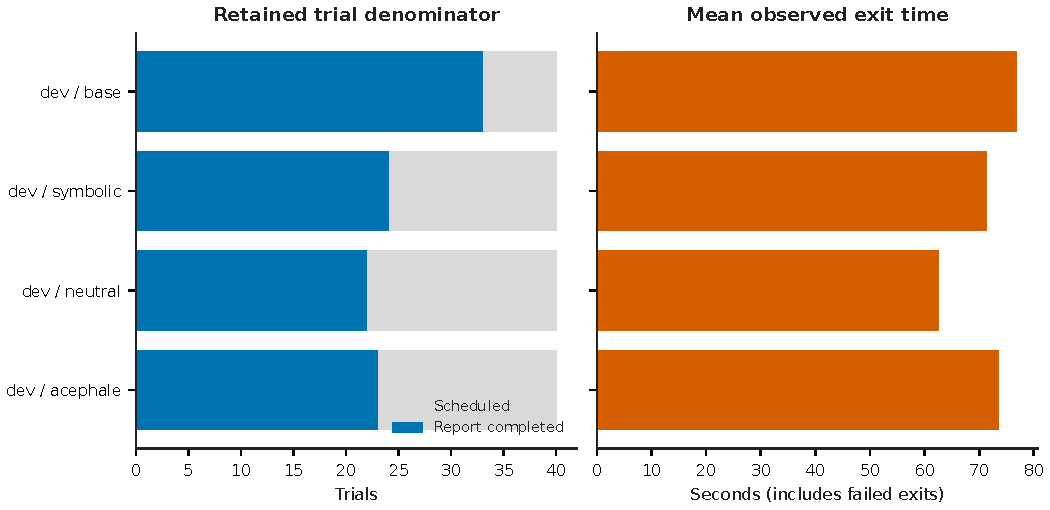
\includegraphics[width=1\textwidth]{figures/outcomes.pdf}
\captionof{figure}{Original final-analysis summaries copied into the plot tables. Bars show retained report completion and observation counts; the timing panel is descriptive, not an uncertainty interval.}
\end{minipage}\end{center}

\hypertarget{primary-comparison-and-uncertainty}{%
\subsection{Primary comparison and uncertainty}\label{primary-comparison-and-uncertainty}}

The primary claim is unavailable under the original gate or complete-pair requirements. This is not a zero effect estimate. Retained reason: development\_gate\_failed.

The original analyzer uses paired question-family clusters, 2,000 bootstrap draws and seed 42. The prospective criterion requires at least 5\% lower mean latency, a latency-saving interval wholly above zero, and a RACE quality-difference interval lower bound of at least -2 points. RACE ratios are multiplied by 100; FACT remains secondary and descriptive. All 100 heldout timing and quality pairs must be complete for the primary claim. No interval is recomputed by the renderer.

\hypertarget{candidate-and-calibration-limitations}{%
\section{Candidate and calibration limitations}\label{candidate-and-calibration-limitations}}

\begin{longtable}[]{@{}
  >{\raggedright\arraybackslash}p{(\columnwidth - 8\tabcolsep) * \real{0.2000}}
  >{\raggedright\arraybackslash}p{(\columnwidth - 8\tabcolsep) * \real{0.2000}}
  >{\raggedright\arraybackslash}p{(\columnwidth - 8\tabcolsep) * \real{0.2000}}
  >{\raggedright\arraybackslash}p{(\columnwidth - 8\tabcolsep) * \real{0.2000}}
  >{\raggedright\arraybackslash}p{(\columnwidth - 8\tabcolsep) * \real{0.2000}}@{}}
\toprule\noalign{}
\begin{minipage}[b]{\linewidth}\raggedright
Population
\end{minipage} & \begin{minipage}[b]{\linewidth}\raggedright
Eligible checkpoints
\end{minipage} & \begin{minipage}[b]{\linewidth}\raggedright
Full-pool hits
\end{minipage} & \begin{minipage}[b]{\linewidth}\raggedright
Window hits
\end{minipage} & \begin{minipage}[b]{\linewidth}\raggedright
Unavailable windows
\end{minipage} \\
\midrule\noalign{}
\endhead
\bottomrule\noalign{}
\endlastfoot
Visit reads & 46 & 0 & 0 & 0 \\
All reads & 86 & 0 & 0 & 0 \\
\end{longtable}

The calibration export retains 98 actor requests, 97 observed label checkpoints and 1 unavailable labels. Observed exact-read labels are evaluated before ranking. The zero-hit calibration population, when present in the table, constrains what any ranker can accomplish on this fixed pool; it is not a proof that goals are useless.

The retained URL audit separates exact invocation mismatches from absence in visible sources. Query-only differences include the actor dropping utm\_source=openai; no URL normalization is applied retrospectively. Original raw provider response bodies were not retained for this audit, so a discarded clean provider URL cannot be established from hashes alone. Calibration maps and score availability remain tied to the declared families and actual closed exports.

\begin{center}\begin{minipage}{\linewidth}
\centering
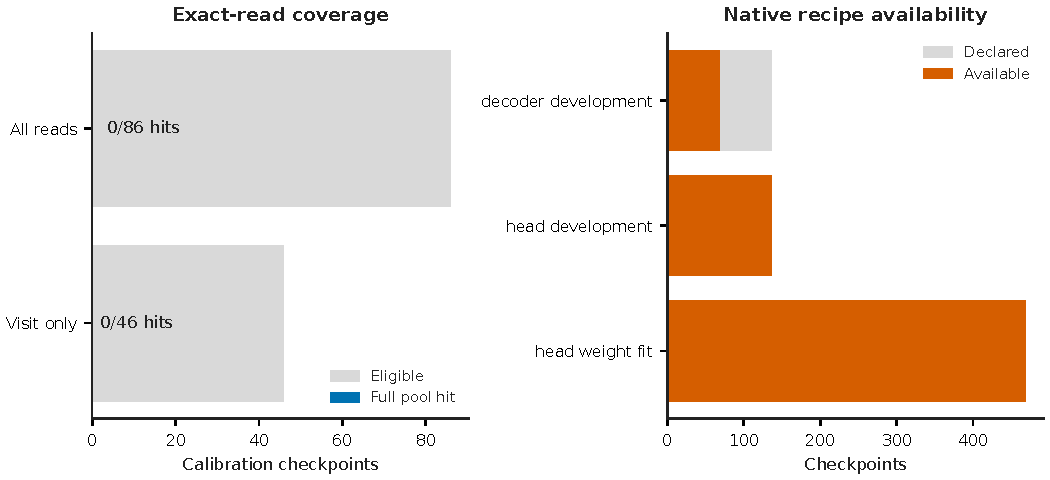
\includegraphics[width=1\textwidth]{figures/coverage.pdf}
\captionof{figure}{Coverage and availability copied from their original reports. Unavailable decoder cases remain in the declared denominator rather than becoming negative labels.}
\end{minipage}\end{center}

\hypertarget{native-prefix-discriminative-head-experiment}{%
\section{Native-prefix discriminative-head experiment}\label{native-prefix-discriminative-head-experiment}}

The separate dataset contains 469 fitting checkpoints across 24 families and 136 development checkpoints. The original generative predictor was trained on 358 complete multitask checkpoints. This 469-versus-358 comparison changes the full recipe and training coverage; it does not isolate head architecture. The frozen-backbone candidate head emits independent logits from context, optional goals and exact candidate representations; the autoregressive decoder's bit probabilities condition on preceding output tokens.

Both native-head recipes use neutral-only examples; this is not a direct test of a goal-conditioned head. The retained recipes use loss weights 0.70 for binary classification, 0.20 for listwise ranking and 0.10 for action prediction; head learning rate 0.0003, backbone learning rate 0.00003, effective batch size 16, three epochs and seed 17. The frozen-backbone variant does not adapt the encoder. The rank-8 variant uses adapter rank 8, alpha 16 and dropout 0.1. Both complete 90 optimizer updates. Development selection uses the same six families, so these results remain exploratory.

Of 136 declared decoder development cases, 68 fit its input budget and 68 are explicitly unavailable. The available set includes 24 empty windows and 44 cases requiring generation. Empty windows are not model-generated successes. Same-panel comparisons must use equivalent visible information where both recipes fit and retain the full availability accounting separately.

The original symbolic proposal order is an essential diagnostic for this native panel:

\begin{longtable}[]{@{}llll@{}}
\toprule\noalign{}
Population & Covered windows & Top1 numerator & Recall3 numerator \\
\midrule\noalign{}
\endhead
\bottomrule\noalign{}
\endlastfoot
All windows & 28 & 24 & 27.000 \\
Generative-available & 16 & 16 & 16.000 \\
Generative-unavailable & 12 & 8 & 11.000 \\
\end{longtable}

Only 11 covered windows contain more than three candidates. These are conditional ranking metrics on covered reads, not action accuracy or task success. The decoder-available subset is easier under proposal order; its results cannot stand in for all136 windows.

The separate checkpoint29 sensitivity replay is physically closed on the exact original research calibration export. Its source-bound raw independent-stage results are retained; it is distinct from the historical native replay and does not change the primary calibration or live control. Checkpoint29 uses the restored, historically qualified seven-file runtime, while primary checkpoint17 used the stock runtime; this is checkpoint/runtime sensitivity, not an isolated training-seed effect.

\hypertarget{frozen-backbone-head}{%
\subsection{Frozen-backbone head}\label{frozen-backbone-head}}

Actual optimizer updates: 90; selected epoch 1. Selection uses this variant's development Recall@3, with binary log loss as tie-break. This is not heldout evaluation, calibration, or selection between the two variants.

\begin{longtable}[]{@{}ll@{}}
\toprule\noalign{}
Trainer-weighted selected metric & Original value \\
\midrule\noalign{}
\endhead
\bottomrule\noalign{}
\endlastfoot
candidateCount & 3.247 \\
positiveCount & 0.186 \\
actionCorrect & 0.711 \\
exactRecallAt1 & 0.824 \\
exactRecallAt3 & 1.000 \\
brier & 0.083 \\
binaryLogLoss & 0.467 \\
\end{longtable}

This original trainer summary uses all-family checkpoint weights renormalized over defined metrics. The comparison below instead reports equal means over families with defined metrics and checkpoint-level means; these estimands must not be interchanged.

All development prefixes: 136/136 available checkpoints; 28 covered reads.

\begin{longtable}[]{@{}llll@{}}
\toprule\noalign{}
Metric & Equal-family mean & Checkpoint mean & N / families \\
\midrule\noalign{}
\endhead
\bottomrule\noalign{}
\endlastfoot
Top1 yield / all prefixes & 0.153 & 0.162 & 136 / 6 \\
Top3 yield / all prefixes & 0.186 & 0.206 & 136 / 6 \\
Binary log loss & 0.456 & 0.509 & 112 / 6 \\
Brier & 0.081 & 0.090 & 112 / 6 \\
Recall3 / covered reads & 1.000 & 1.000 & 28 / 6 \\
Top1 / covered reads & 0.903 & 0.786 & 28 / 6 \\
Top1 hit / eligible reads & 0.404 & 0.423 & 52 / 6 \\
Top3 hit / eligible reads & 0.481 & 0.538 & 52 / 6 \\
Recorded head action accuracy & 0.711 & 0.699 & 136 / 6 \\
\end{longtable}

Generative-available subset: 68/136 available checkpoints; 16 covered reads.

\begin{longtable}[]{@{}llll@{}}
\toprule\noalign{}
Metric & Equal-family mean & Checkpoint mean & N / families \\
\midrule\noalign{}
\endhead
\bottomrule\noalign{}
\endlastfoot
Top1 yield / all prefixes & 0.237 & 0.221 & 68 / 6 \\
Top3 yield / all prefixes & 0.257 & 0.235 & 68 / 6 \\
Binary log loss & 1.179 & 0.830 & 44 / 6 \\
Brier & 0.239 & 0.157 & 44 / 6 \\
Recall3 / covered reads & 1.000 & 1.000 & 16 / 5 \\
Top1 / covered reads & 0.950 & 0.938 & 16 / 5 \\
Top1 hit / eligible reads & 0.490 & 0.484 & 31 / 6 \\
Top3 hit / eligible reads & 0.532 & 0.516 & 31 / 6 \\
Recorded head action accuracy & 0.685 & 0.706 & 68 / 6 \\
\end{longtable}

Head minus symbolic (exploratory paired family intervals):

\begin{longtable}[]{@{}lll@{}}
\toprule\noalign{}
Metric & Difference & 95\% interval \\
\midrule\noalign{}
\endhead
\bottomrule\noalign{}
\endlastfoot
Top1 yield / all prefixes & -0.013 & {[}-0.030, 0.000{]} \\
Top3 yield / all prefixes & 0.005 & {[}0.000, 0.015{]} \\
Recall3 / covered reads & 0.014 & {[}0.000, 0.042{]} \\
Top1 / covered reads & -0.042 & {[}-0.097, 0.000{]} \\
Top1 hit / eligible reads & -0.032 & {[}-0.074, 0.000{]} \\
Top3 hit / eligible reads & 0.011 & {[}0.000, 0.033{]} \\
\end{longtable}

Head minus generative (exploratory paired family intervals):

\begin{longtable}[]{@{}lll@{}}
\toprule\noalign{}
Metric & Difference & 95\% interval \\
\midrule\noalign{}
\endhead
\bottomrule\noalign{}
\endlastfoot
Top1 yield / all prefixes & 0.021 & {[}-0.062, 0.125{]} \\
Top3 yield / all prefixes & 0.021 & {[}0.000, 0.062{]} \\
Binary log loss & -4.383 & {[}-5.676, -2.596{]} \\
Brier & -0.240 & {[}-0.430, -0.081{]} \\
Recall3 / covered reads & 0.050 & {[}0.000, 0.150{]} \\
Top1 / covered reads & 0.050 & {[}-0.150, 0.300{]} \\
Top1 hit / eligible reads & 0.042 & {[}-0.125, 0.250{]} \\
Top3 hit / eligible reads & 0.042 & {[}0.000, 0.125{]} \\
\end{longtable}

These intervals are exploratory: the same development families selected each variant's epoch. Differences are head minus comparator; lower Brier and log loss are better, while higher hit/recall yields are better. Recorded head action accuracy is not task reward or goal agreement.

This variant's source-bound whole-recipe comparison is retained separately. Read its actual matched intersection together with all136-case availability; neither variant is selected as a winner here.

\hypertarget{rank-8-adapter-head}{%
\subsection{Rank-8 adapter head}\label{rank-8-adapter-head}}

Actual optimizer updates: 90; selected epoch 3. Selection uses this variant's development Recall@3, with binary log loss as tie-break. This is not heldout evaluation, calibration, or selection between the two variants.

\begin{longtable}[]{@{}ll@{}}
\toprule\noalign{}
Trainer-weighted selected metric & Original value \\
\midrule\noalign{}
\endhead
\bottomrule\noalign{}
\endlastfoot
candidateCount & 3.247 \\
positiveCount & 0.186 \\
actionCorrect & 0.774 \\
exactRecallAt1 & 0.745 \\
exactRecallAt3 & 1.000 \\
brier & 0.072 \\
binaryLogLoss & 0.237 \\
\end{longtable}

This original trainer summary uses all-family checkpoint weights renormalized over defined metrics. The comparison below instead reports equal means over families with defined metrics and checkpoint-level means; these estimands must not be interchanged.

All development prefixes: 136/136 available checkpoints; 28 covered reads.

\begin{longtable}[]{@{}llll@{}}
\toprule\noalign{}
Metric & Equal-family mean & Checkpoint mean & N / families \\
\midrule\noalign{}
\endhead
\bottomrule\noalign{}
\endlastfoot
Top1 yield / all prefixes & 0.139 & 0.140 & 136 / 6 \\
Top3 yield / all prefixes & 0.186 & 0.206 & 136 / 6 \\
Binary log loss & 0.232 & 0.255 & 112 / 6 \\
Brier & 0.070 & 0.078 & 112 / 6 \\
Recall3 / covered reads & 1.000 & 1.000 & 28 / 6 \\
Top1 / covered reads & 0.861 & 0.679 & 28 / 6 \\
Top1 hit / eligible reads & 0.371 & 0.365 & 52 / 6 \\
Top3 hit / eligible reads & 0.481 & 0.538 & 52 / 6 \\
Recorded head action accuracy & 0.774 & 0.750 & 136 / 6 \\
\end{longtable}

Generative-available subset: 68/136 available checkpoints; 16 covered reads.

\begin{longtable}[]{@{}llll@{}}
\toprule\noalign{}
Metric & Equal-family mean & Checkpoint mean & N / families \\
\midrule\noalign{}
\endhead
\bottomrule\noalign{}
\endlastfoot
Top1 yield / all prefixes & 0.195 & 0.191 & 68 / 6 \\
Top3 yield / all prefixes & 0.257 & 0.235 & 68 / 6 \\
Binary log loss & 0.639 & 0.454 & 44 / 6 \\
Brier & 0.206 & 0.141 & 44 / 6 \\
Recall3 / covered reads & 1.000 & 1.000 & 16 / 5 \\
Top1 / covered reads & 0.850 & 0.812 & 16 / 5 \\
Top1 hit / eligible reads & 0.407 & 0.419 & 31 / 6 \\
Top3 hit / eligible reads & 0.532 & 0.516 & 31 / 6 \\
Recorded head action accuracy & 0.772 & 0.824 & 68 / 6 \\
\end{longtable}

Head minus symbolic (exploratory paired family intervals):

\begin{longtable}[]{@{}lll@{}}
\toprule\noalign{}
Metric & Difference & 95\% interval \\
\midrule\noalign{}
\endhead
\bottomrule\noalign{}
\endlastfoot
Top1 yield / all prefixes & -0.028 & {[}-0.067, 0.000{]} \\
Top3 yield / all prefixes & 0.005 & {[}0.000, 0.015{]} \\
Recall3 / covered reads & 0.014 & {[}0.000, 0.042{]} \\
Top1 / covered reads & -0.083 & {[}-0.194, 0.000{]} \\
Top1 hit / eligible reads & -0.065 & {[}-0.154, 0.000{]} \\
Top3 hit / eligible reads & 0.011 & {[}0.000, 0.033{]} \\
\end{longtable}

Head minus generative (exploratory paired family intervals):

\begin{longtable}[]{@{}lll@{}}
\toprule\noalign{}
Metric & Difference & 95\% interval \\
\midrule\noalign{}
\endhead
\bottomrule\noalign{}
\endlastfoot
Top1 yield / all prefixes & -0.021 & {[}-0.125, 0.062{]} \\
Top3 yield / all prefixes & 0.021 & {[}0.000, 0.062{]} \\
Binary log loss & -4.923 & {[}-6.570, -2.835{]} \\
Brier & -0.273 & {[}-0.434, -0.151{]} \\
Recall3 / covered reads & 0.050 & {[}0.000, 0.150{]} \\
Top1 / covered reads & -0.050 & {[}-0.300, 0.150{]} \\
Top1 hit / eligible reads & -0.042 & {[}-0.250, 0.125{]} \\
Top3 hit / eligible reads & 0.042 & {[}0.000, 0.125{]} \\
\end{longtable}

These intervals are exploratory: the same development families selected each variant's epoch. Differences are head minus comparator; lower Brier and log loss are better, while higher hit/recall yields are better. Recorded head action accuracy is not task reward or goal agreement.

This variant's source-bound whole-recipe comparison is retained separately. Read its actual matched intersection together with all136-case availability; neither variant is selected as a winner here.

\hypertarget{original-fast-tool-negative-control}{%
\section{Original fast-tool negative control}\label{original-fast-tool-negative-control}}

The November22 study retains all36 development and96 heldout trials. It is reported separately and is not relabeled as research-protocol05 evidence. No prefetch benefit was demonstrated; zero actual speculative exposure prevents a claim about the efficacy of executed prefetch. The old task metrics are custom tau-compatible, unofficial results \citep{tau2paper, tau2pinned}. Database reward, constraint cleanliness and exact-read prediction are distinct outcomes. The old reports, paper and failures remain immutable.

\hypertarget{interpretation-and-limitations}{%
\section{Interpretation and limitations}\label{interpretation-and-limitations}}

The source-bound development error audit retains 49 error rows. Of these, 40 record cleanup ConnectError and an undrained trial status. These operational failures must not be attributed solely to predictor quality. Later outer process-cleanup receipts establish subsequent shutdown; they do not change the original per-trial undrained metadata or turn failed rows into successes. The reproduction manifest retains the original audit digest.

An inferred goal computed from the same public prefix is an additional representation for a finite predictor, not guaranteed new information. It may help a limited predictor or retrieval procedure, but can add estimation error and execution overhead. This is a mechanism argument, not an observed causal result.

The study distinguishes four failure locations: the desired invocation is absent from the public pool; a represented candidate is misranked; a proposed read fails admission or freshness; or a valid speculative read does not reduce whole-task latency without reducing quality. Negative results at an earlier location limit the interpretation of later mechanisms. We do not infer task quality from an actor ending its report or source validity from a plausible URL.

The research questions use lexical family separation, which does not establish perfect semantic independence. The historical annotation audit has zero human reviews and uses the same hosted model in separate teacher/reviewer requests. Hosted usage estimates, reserved budgets and provider invoices are different quantities. Missing or unknown costs are not zero. This is a custom pinned evaluation with declared adaptations, not an official unmodified benchmark or a state-of-the-art claim.

\hypertarget{related-work-and-source-provenance}{%
\section{Related work and source provenance}\label{related-work-and-source-provenance}}

The retained version-specific bibliography accompanies this manuscript. Tool/generation overlap follows the problem studied by PASTE; historical retrieval follows Speculate with Memory. This work adds source-bound goal conditioning and separates coverage, availability, admission and task-level effects.

The retained versions are PASTE \citep{sui2026paste} and Speculate with Memory \citep{li2026memory}.

\begingroup\footnotesize\setlength{\parskip}{0pt}\setlength{\bibsep}{3pt plus 1pt minus 1pt}
\bibliographystyle{plainnat}
\bibliography{references}
\endgroup
\end{document}
